\chapter{Methods}

This chapter will outline the methods how SCVAEs and non-conditioned VAEs are
integrated using multitask learning in this thesis. Initially, describe the
method of merging SCVAEs with non-conditioned VAEs by expanding the SCVAEs
framework with a second decoder. This method will be applied to both Gaussian
VAEs and VQ-VAEs. In the following section, I will describe another method of
merging SCVAEs with non-conditioned VAEs by utilizing the same encoder and
decoder for both models by employing novel training strategies. This method
will also be applied to both Gaussian VAEs and VQ-VAEs.


\section{\method{1}}

In the first method, we expand the VAEs framework with a second decoder
$p_\xi(x|z,m)$, which is conditioned on an additional property $m$ of the input
data. This approach involves utilizing two decoders within the VAEs framework:
one for reconstructing the input data solely based on the latent variable $z$,
and the other for reconstructing the input data based on both the latent
variable $z$ and the additional conditioning information $m$.

\subsection{Conditioning information}

In this method, the conditioning information $m$ is acquired by sampling
constant number of pixels from the input data. To sample the pixels from the
input image $x$, we will use a pixel sampling operation, which will be
described in the following section.

\subsubsection{Pixel Sampling operation}

To acquire the conditioning information $m$ from the input image $x$, we will
use sampling operation. I will explore two sampling types for this method,
which can be seen in Figure~\ref{SamplingFigure} and are described as follows:

\begin{enumerate}
    \item \textbf{Exact same sampling:} In this sampling type, the conditioning information $m$ is sampled from the input image $x$ by sampling the exact same sparse pixels from the input image $x$. In this work, the pixels that will be sampled from the input image will be a sparse grid of pixels.
    \item \textbf{Uniform random sampling:} In this sampling type, the conditioning information $m$ is sampled from the input image $x$ by sampling exact number of pixels from the input image $x$ uniformly at random.
\end{enumerate}

\subsection{Application to Gaussian VAEs}

In Gaussian VAEs, the integration of a second conditioned decoder
$p_\xi(x|z,m)$ follows a similar approach as outlined in the general method
description. However, there are specific adjustments and considerations that
need to be taken into account when applying this method to Gaussian VAEs.

The integration of the second conditioned decoder $p_\xi(x|z,m)$ into the
Gaussian VAEs framework involves using a fully connected layer to merge the
latent variable $z$ and the conditioning information $m$ before passing it
through the transposed convolutional layers. The architecture of the Gaussian
VAEs framework with the second conditioned decoder is illustrated in
Figure~\ref{SCVAE2DFigure}

In Gaussian VAEs, the loss objective consists of two components: the
reconstruction loss and the KL divergence term. However, with the inclusion of
the second conditioned decoder, the loss objective is extended to include the
reconstruction loss of the second conditioned decoder. The overall loss
objective to be \textbf{minimized} becomes

\[ L = \frac{1}{D} \sum_{i=1}^{D} ||x_i - \hat{x}_1 ||^2 + \frac{1}{D} \sum_{i=1}^{D} || x_i - \hat{x}_2 ||^2 + \beta  \frac{1}{2} \biggl( -\log \sigma^2_\phi(x) - 1 + \mu^2_\phi(x) + \sigma^2_\phi(x) \biggr), \]

where $D$ is the number of pixels in the input image, $x_i$ is the $i$-th pixel
of the input image, $\hat{x}_1$ is the output of the first decoder, $\hat{x}_2$
is the output of the second decoder, $\beta$ is the KL divergence weight,
$\mu_\phi(x)$ and $\sigma_\phi(x)$ are the mean and the standard deviation of
the Gaussian distribution produced by the encoder, respectively.

During the training process, the encoder is trained to produce accurate mean
and standard deviation of the Gaussian distribution, and the decoders are
trained to produce accurate reconstructions of the input data. The KL
divergence term is used to regularize the latent space to be close to a
standard Gaussian distribution. The optimizer used to minimize the overall loss
objective is the AdamW optimizer~\cite{AdamW}.

As a result of the integration of the second conditioned decoder, the model has
the ability to reconstruct the input data based just on the latent variable $z$
and as well as the conditioning information $m$.
\begin{figure}[H]
    \centering
    \centering
\scriptsize
\begin{tabular}{||c|c|c|c||}
\hline
 Method & Parameters & Reconstruction loss & KL loss \\
\hline
\textit{Baseline} & - & 0.0042 +- 1.2e-03 & 0.0018 +- 6.3e-04 \\
\hline
Multi Decoder & Exact sampling & 0.0036 +- 8.3e-04  $\downarrow$ & 0.0027 +- 8.7e-04  $\uparrow$ \\
\hline
Multi Decoder & Exact sampling, SoftAdapt & 0.0034 +- 1.9e-04  $\downarrow$ & 0.0029 +- 2.8e-03  $\uparrow$ \\
\hline
Multi Decoder & Uniform sampling & 0.0035 +- 6.5e-04  $\downarrow$ & 0.0026 +- 1.7e-03  $\uparrow$ \\
\hline
Multi Decoder & Uniform sampling, SoftAdapt & 0.0034 +- 7.3e-03  $\downarrow$ & 0.0029 +- 2.0e-02  $\uparrow$ \\
\hline
\end{tabular}

    \caption[\method{1} applied to Gaussian VAEs.]%
    {
        \methodOne\ applied to Gaussian VAEs. The Gaussian VAEs framework is extended by adding a second conditioned decoder $p_\xi(x|z,m)$. The input $x$ is passed through the encoder with parameters $\phi$ producing the mean $\mu$ and the standard deviation $\sigma$ of the Gaussian distribution. The random variable $\epsilon$ is sampled from a standard Gaussian distribution and is used to sample $ z = \mu + \sigma \odot \epsilon$. The sampled $z$ is then used as input to both decoders. As a result, the loss function consists of three components: the MSE reconstruction loss of the first decoder, the MSE reconstruction loss of the second decoder and the KL divergence regularization loss.
    }\label{SCVAE2DFigure}
\end{figure}

\subsection{Application to VQ-VAEs}

The approach of integrating the second conditioned decoder $p_\xi(x|z,m)$ into
the VQ-VAEs framework is similar to the approach used for Gaussian VAEs.
However, there differences that need to be taken into account when applying
this method to VQ-VAEs.

The VQ-VAEs differ from the Gaussian VAEs in that the VQ-VAEs use Vector
Quantization to discretize the continuous latent space. Because of this, the
latent variable $z$ can not be directly merged with the conditioning
information $m$ using a fully connected layer. Instead,

One of the main differences is that the VQ-VAEs framework uses a discrete
latent space and the Vector Quantization. Because of this, the latent variable
$z$ can not be directly merged with the conditioning information $m$ using a
fully connected layer. Instead, the corresponding embedding table vectors
$z_q(x)$ must be computed for the latent variable $z$ before merging it with
the conditioning information $m$. The architecture of the VQ-VAEs framework
with the second conditioned decoder is illustrated in
Figure~\ref{SCVQVAE2DFigure}.

In VQ-VAEs, the loss objective consists of three components: the MSE
reconstruction loss and the commitment loss and the codebook loss. However,
with the inclusion of the second conditioned decoder, the loss objective is
extended to include the reconstruction loss of the second conditioned decoder.
The overall loss objective to be \textbf{minimized} becomes

\[ L = \frac{1}{D} \sum_{i=1}^{D} ||x_i - \hat{x}_1 ||^2 + \frac{1}{D} \sum_{i=1}^{D} || x_i - \hat{x}_2 \hat{x} ||^2 + || sg(z_e(x)) - e_k ||^2 + \beta || z_q(x) - sg(e_k) ||^2 , \]

where $D$ is the number of pixels in the input image, $x_i$ is the $i$-th pixel
of the input image, $\hat{x}_1$ is the output of the first decoder, $\hat{x}_2$
is the output of the second decoder, $z_e(x)$ is the output of the encoder,
$z_q(x)$ is the mapping output after Vector Quantization, $e_k$ is the $k$-th
embedding table vector, $\beta$ is the commitment loss weight, $sg$ is the stop
gradient operation.

After the first stage of the training, the model has the ability to reconstruct
the input data based just on the latent variable $z$ and as well as the
conditioning information $m$. To generate the latent variable $z$ there must be
trained a separate autoregressive model, which will be used to generate the
latent variable $z$.

\begin{figure}[H]
    \centering
    \centering
\scriptsize
\begin{tabular}{||c|c|c|c||}
\hline
 Method & Parameters & Reconstruction loss & VQ loss \\
\hline
\textit{Baseline} & - & 0.0022 +- 7.4e-08 & 0.0029 +- 4.1e-07 \\
\hline
Multi Decoder & Exact sampling & 0.0017 +- 6.9e-09  $\downarrow$ & 0.0039 +- 9.8e-07  $\uparrow$ \\
\hline
Multi Decoder & Exact sampling, SoftAdapt & \textbf{0.0013 +- 2.4e-09}  $\downarrow$ & \textbf{0.0016 +- 6.8e-08}  $\downarrow$ \\
\hline
Multi Decoder & Uniform sampling & 0.0018 +- 1.3e-07  $\downarrow$ & 0.0036 +- 3.5e-07  $\uparrow$ \\
\hline
Multi Decoder & Uniform sampling, SoftAdapt & \textbf{0.0017 +- 6.6e-08}  $\downarrow$ & \textbf{0.0021 +- 3.1e-07}  $\downarrow$ \\
\hline
\end{tabular}

    \caption[\method{1} applied to VQ-VAEs.]%
    {
        \method{1} applied to VQ-VAEs. The VQ-VAEs framework is extended by adding a second conditioned decoder. Instead of using a fully connected layer to merge the latent variable $z$ and the conditioning information $m$, the corresponding embedding table vectors $z_q(x)$ must be computed for the latent variable $z$ before merging it with the conditioning information $m$. As a result of adding the second conditioned decoder, the loss function requires the addition of the MSE reconstruction loss of the second decoder.
    }\label{SCVQVAE2DFigure}
\end{figure}

\section{\method{2}}

In the second method, I use a single decoder within the VAE Architecture.
However, the use decoder is expanded to be capable of reconstructing the input
data under variable conditioning. The variable conditioning means that the
conditioning information $m$ can be a variable amount of information or just an
empty mask.

This method utilizes a single decoder that dynamically adjusts its behavior
based on the amount of information present in the variable $m$. When the
conditioning information is available, the decoder incorporates it into the
reconstruction process and takes advantage of it to get the best
reconstruction. Otherwise, it operates solely based on the latent variable $z$.

\subsection{Conditioning strategy}

Similar to the previous method, the conditioning information $m$ is acquired by sampling pixels from the input image $x$. However, in this method, the conditioning information $m$ is sampled by selecting a variable number of pixels from the input image $x$. The number of pixels to be sampled from the input image varies and is sampled from a power law distribution. The power law distribution is scaled to the size of the input image $x$ and is used to compute the number of pixels to be sampled from the input image $x$.

The conditioning information $m$ includes an additional mask, which indicates to the decoder which pixels are sampled from the input image $x$ and which pixels are not sampled. The mask is a binary matrix of the same size as the input image $x$, where a value of 1 represents the sampled pixels and a value of 0 represents the pixels that are not sampled. When there is no conditioning information, the mask is filled with zeros. If image $x$ has 3 channels, then the mask will be applied to all channels. The count sampling distribution is chosen to be a power law distribution with a high exponent so that the decoder can learn to handle also the cases where the conditioning information is not available. The exponent will be a hyperparameter of the model.

For the conditioning information $m$, I will implement a two-step sampling process:

\begin{enumerate}
    \item \textbf{Sampling the number of pixels:} In this step, the number of pixels to be sampled from the input image $x$ is sampled from a power law distribution. The power law distribution is scaled to the size of the input image $x$ and is used to sample the number of pixels to be sampled from the input image $x$.
    \item \textbf{Sampling the pixels:} In this step, the conditioning information $m$ is sampled from the input image $x$ by sampling the number of pixels sampled in the previous step from the input image $x$ uniformly at random or from a Gaussian distribution, which can be seen in Figure~\ref{SamplingFigure}.
\end{enumerate}

\subsection{Application to Gaussian VAEs}

In Gaussian VAEs, applying the second method involves modifying the decoder to be capable of reconstructing the input data under variable conditioning. The modified decoder $p_\xi(x|z,m)$ is capable of reconstructing the input data based on the latent variable $z$ and the conditioning information $m$ or just the latent variable $z$.

This is achieved by using a fully connected layer to merge the latent variable $z$ and the conditioning information $m$ before passing it through the transposed convolutional layers. The architecture of the Gaussian VAEs framework with a single decoder capable of variable conditioning is illustrated in Figure~\ref{SCVAE1DFigure}.



\begin{figure}[H]
    \centering
    \centering
\scriptsize
\begin{tabular}{||c|c|c|c||}
\hline
 Method & Parameters & Reconstruction loss & KL loss \\
\hline
\textit{Baseline} & - & 0.0097 +- 4.2e-03 & 63.0518 +- 2.4e+01 \\
\hline
Single Decoder & Gaussian sampling, Exponent=40 & 0.0113 +- 1.4e-02  $\uparrow$ & 54.7483 +- 7.3e+01  $\downarrow$ \\
\hline
Single Decoder & Gaussian sampling, Exponent=60 & 0.0113 +- 2.6e-03  $\uparrow$ & 54.6946 +- 4.4e+01  $\downarrow$ \\
\hline
\end{tabular}

    \caption[\method{2} applied to Gaussian VAEs.]%
    {
        \methodTwo\ applied to Gaussian VAEs. The Gaussian VAEs framework is modified by allowing the decoder to be conditioned on a variable amount of information and to dynamically adjust its behavior based on the amount of information present in the variable $m$. The input $x$ is passed through the encoder with parameters $\phi$ producing the mean $\mu$ and the standard deviation $\sigma$ of the Gaussian distribution. The random variable $\epsilon$ is sampled from a standard Gaussian distribution and is used to sample $ z = \mu + \sigma \odot \epsilon$. The sampled $z$ is then used as input to the decoder as well as the extra conditioning information $m$. With this approach there is no need for a second decoder, as the single decoder is capable to reconstruct the data based on the latent variable $z$ and the conditioning information $m$ or just the latent variable $z$.
    }\label{SCVAE1DFigure}
\end{figure}

\subsection{Application to VQ-VAEs}

In VQVAEs, same as in Gaussian VAEs, the second method involves modifying the decoder to be capable to receive variable conditioning information. Unlike Gaussian VAEs, the VQ-VAEs use Vector Quantization to discretize the continuous latent space. Because of this, the latent variable $z$ can not be directly merged with the conditioning information $m$ using a fully connected layer. Instead, the corresponding embedding table vectors $z_q(x)$ must be computed for the latent variable $z$ before merging it with the conditioning information $m$. The architecture of the VQ-VAEs framework with a single decoder capable of variable conditioning is illustrated in Figure~\ref{SCVQVAE1DFigure}.

\begin{figure}[H]
    \centering
    \centering
\scriptsize
\begin{tabular}{||c|c|c|c||}
\hline
 Method & Parameters & Reconstruction loss & VQ loss \\
\hline
\textit{Baseline} & - & 0.0022 +- 4.2e-08 & 0.0048 +- 8.3e-07 \\
\hline
Single Decoder & Gaussian sampling, Exponent=40 & 0.0026 +- 1.9e-07  $\uparrow$ & 0.0028 +- 2.3e-06  $\downarrow$ \\
\hline
Single Decoder & Gaussian sampling, Exponent=40 & 0.0023 +- 3.9e-07  $\uparrow$ & 0.0015 +- 7.3e-08  $\downarrow$ \\
\hline
Single Decoder & Gaussian sampling, Exponent=60 & 0.0029 +- 4.5e-07  $\uparrow$ & 0.0041 +- 4.1e-06  $\downarrow$ \\
\hline
Single Decoder & Gaussian sampling, Exponent=60 & \textbf{0.0020 +- 9.2e-08}  $\downarrow$ & \textbf{0.0013 +- 7.6e-08}  $\downarrow$ \\
\hline
Single Decoder & Uniform sampling, Exponent=40 & \textbf{0.0022 +- 1.1e-08}  $\downarrow$ & \textbf{0.0020 +- 2.2e-08}  $\downarrow$ \\
\hline
Single Decoder & Uniform sampling, Exponent=40 & \textbf{0.0022 +- 1.2e-07}  $\downarrow$ & \textbf{0.0018 +- 1.1e-08}  $\downarrow$ \\
\hline
Single Decoder & Uniform sampling, Exponent=60 & 0.0026 +- 7.2e-08  $\uparrow$ & 0.0030 +- 8.0e-07  $\downarrow$ \\
\hline
Single Decoder & Uniform sampling, Exponent=60 & 0.0023 +- 2.1e-07  $\uparrow$ & 0.0015 +- 9.0e-08  $\downarrow$ \\
\hline
\end{tabular}

    \caption[\method{2} applied to VQ-VAEs.]%
    {
        \methodTwo\ applied to VQ-VAEs. The VQ-VAEs framework is modified by allowing the decoder to be conditioned on a variable amount of information and to dynamically adjust its behavior based on the amount of information present in the variable $m$. The input $x$ is passed through the encoder producing the output $z_e(x)$. The output $z_e(x)$ is then used as input to the autoregressive model to generate the latent variable $z$. The latent variable $z$ is then used as input to the decoder as well as the extra conditioning information $m$. With this approach there is no need for a second decoder, as the single decoder is capable to reconstruct the data based on the latent variable $z$ and the conditioning information $m$ or just the latent variable $z$.
    }\label{SCVQVAE1DFigure}
\end{figure}


\begin{figure}
    \centering
    

\tikzset{every picture/.style={line width=0.75pt}} %set default line width to 0.75pt        

\begin{tikzpicture}[x=0.75pt,y=0.75pt,yscale=-1,xscale=1]
%uncomment if require: \path (0,374); %set diagram left start at 0, and has height of 374

%Image [id:dp9293884018723756] 
\draw (365.67,295.2) node  {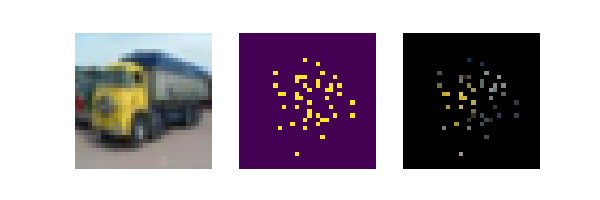
\includegraphics[width=225pt,height=75pt]{figures/assets/GAUSSIAN.png}};
%Image [id:dp548757972749888] 
\draw (365.67,208.8) node  {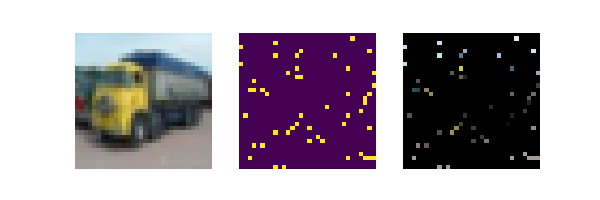
\includegraphics[width=225pt,height=75pt]{figures/assets/UNIFORM.png}};
%Image [id:dp620494998311241] 
\draw (365.67,124.8) node  {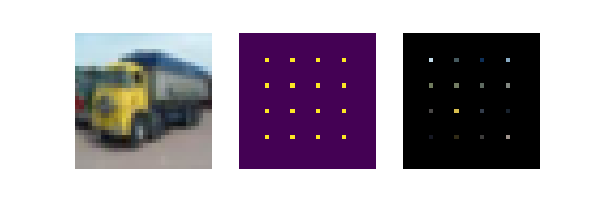
\includegraphics[width=225pt,height=75pt]{figures/assets/EXACT.png}};
%Shape: Grid [id:dp3074430629490833] 
\draw  [draw opacity=0] (242.67,82.33) -- (497.67,82.33) -- (497.67,337.67) -- (242.67,337.67) -- cycle ; \draw   (242.67,82.33) -- (242.67,337.67)(327.67,82.33) -- (327.67,337.67)(412.67,82.33) -- (412.67,337.67)(497.67,82.33) -- (497.67,337.67) ; \draw   (242.67,82.33) -- (497.67,82.33)(242.67,167.33) -- (497.67,167.33)(242.67,252.33) -- (497.67,252.33)(242.67,337.33) -- (497.67,337.33) ; \draw    ;

% Text Node
\draw (279.26,61.29) node [anchor=north west][inner sep=0.75pt]  [rotate=-308.3] [align=left] {original};
% Text Node
\draw (172.67,120) node [anchor=north west][inner sep=0.75pt]   [align=left] {Exact};
% Text Node
\draw (359.26,61.29) node [anchor=north west][inner sep=0.75pt]  [rotate=-308.3] [align=left] {original};
% Text Node
\draw (437.53,61.29) node [anchor=north west][inner sep=0.75pt]  [rotate=-308.3] [align=left] {original};
% Text Node
\draw (165.17,204) node [anchor=north west][inner sep=0.75pt]   [align=left] {Uniform};
% Text Node
\draw (160.17,291) node [anchor=north west][inner sep=0.75pt]   [align=left] {Gaussian};


\end{tikzpicture}

    \caption[Table of pixel sampling types for conditioning.]%
    {
        Table of pixel sampling types for conditioning. The table has 3 rows each representing a different sampling type. The first row represents the exact same sampling type, the second row represents the uniform random sampling type and the third row represents the Gaussian sampling type where the pixels are more likely to be sampled from the center of the image. The first column represents the original image, the second column represents the mask and the third column represents the result of the sampling operation.
    }\label{SamplingFigure}
\end{figure}


